\documentclass[a4paper,12pt]{article}

\usepackage[T1]{fontenc}
\usepackage[utf8]{inputenc}
\usepackage[francais]{babel}
\usepackage{multirow,array}
\usepackage{graphicx}
\usepackage{a4wide}
\newcommand{\HRule}{\rule{\linewidth}{1mm}}

\begin{document}


%
%  TITRE
%

\begin{titlepage}

\begin{center}
\huge Localisation géométrique rapide \\ par arbre octal
\HRule \\
\medskip
{\Huge \bfseries La librairie libOL} \\
\HRule
\end{center}

\vspace*{\stretch{3}}

\begin{figure}[htbp]
\begin{center}
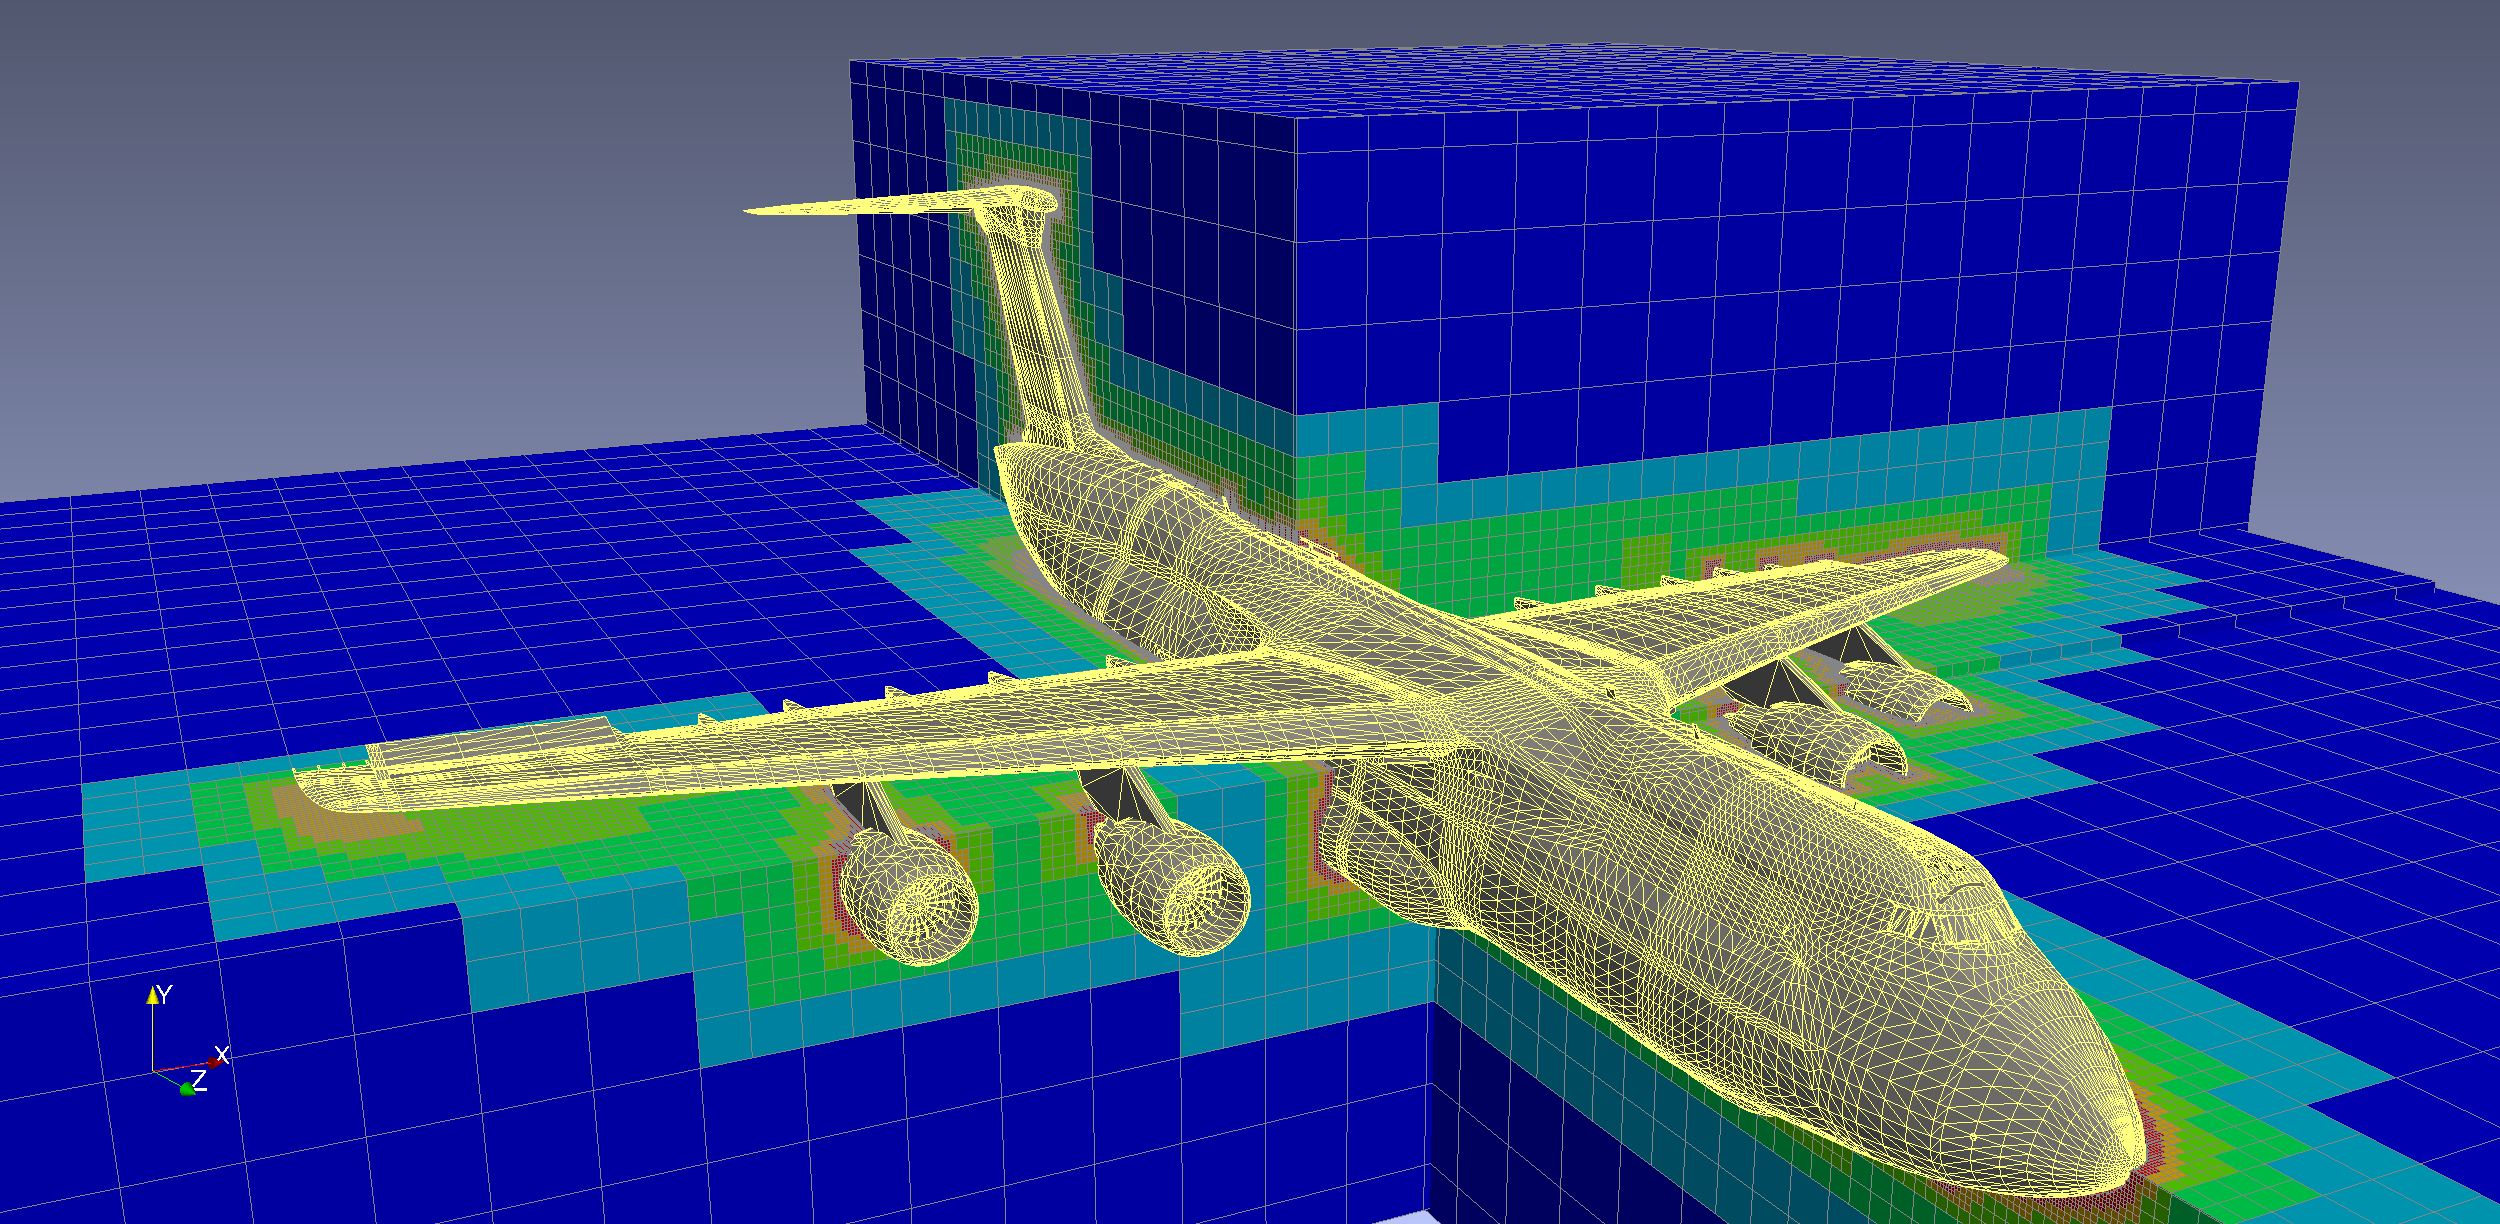
\includegraphics[height=7.8cm]{octree_mesh.png}
\end{center}
\end{figure}

\vspace*{\stretch{1}}

\begin{flushright}
\Large Lo\"ic MAR\'ECHAL / INRIA, Projet Gamma\\
\Large Mars 2016 \\
\normalsize Document v1.2
\end{flushright}

\end{titlepage}

\clearpage

\setcounter{tocdepth}{2}
\tableofcontents
\vfill

\footnotesize{Couverture : Maillage octree d'un Boeing 747 réalisé par Thomas Døhlen.}
\normalsize

\clearpage


%
%  1 / INTRODUCTION
%

\section{Introduction}
Le but de cette librairie est de facilement et rapidement retrouver les éléments d'un maillage à partir de coordonnées géométriques tel que, par exemple, trouver le triangle le plus proche d'un point donné, ou bien de fournir la liste des triangles ou sommets intersectant une région donnée.

D'autres entités que les triangles ou sommets sont prévues telles que les arêtes, les maillages volumiques et les champs de valeurs scalaires ou vectorielles (métriques ou solutions physiques).

Des opérations telles que les distances de triangle à triangle, la localisation d'un sommet dans un tétraèdre ou les lissages de métriques sont prévues.



%
%  2 / UTILISATION
%

\section{Utilisation}
La donnée à fournir à la librairie est un maillage de surface sous sa forme la plus simple : une liste de coordonnées de chaque sommet et une table des numéros des sommets pour chaque triangle. À partir de ce maillage, la librairie génère un octree automatiquement raffiné de telle sorte que chaque octant ne contient au plus que 20 entités de chaque type afin d'accélérer les opérations de recherche. Le temps de construction et la mémoire requis sont donc dépendants du nombre d'entités du maillage et de la forme de la géométrie. Un octree étant fondamentalement isotrope, il aura tendance à être fortement raffiné, et donc à occuper beaucoup de mémoire, dans le cas de géométries très minces (anisotropes).

Bien qu'une structure octree ne contienne qu'un seul maillage, il est possible d'en créer plusieurs, ceux-ci étant différenciés par une étiquette unique retournée à la création.

Supposons que nous avons un maillage de \emph{NmbVer} sommets, stockés dans la table \emph{VerCrd} et \emph{NmbTri} triangles dans la table \emph{TriTab} et que l'on souhaite trouver le triangle le plus proche du point de coordonnées $\{0.5, 2.3, -6.0\}$ ainsi que la liste des triangles contenus partiellement ou totalement dans la région cubique centrée en $\{2,2,10\}$ et de taille $2$. Le déroulement est le suivant :

\begin{tt}
\begin{verbatim}
long long OctIdx;
int IntersectedTriangles[10];
int NmbVer, NmbTri, (*TriTab)[3];
double (*CrdTab)[3], VerCrd[3]={0.5, 2.3, -6.0};
double BoxMin[3]={1,1,9}, BoxMax[3]={3,3,11}, MinDis;
...
(allocation et lecture du maillage)
...
OctIdx = NewOctree(NmbVer, VerTab[1], VerTab[2], NmbTri, TriTab[1], TriTab[1]);
printf("l'Octree numéro %d a été construit\n", OctIdx);

TriIdx = GetNearest(OctIdx, TypTri, VerCrd, &MinDis, 0);
printf("le triangle le plus proche de 0.5, 2.3, -6.0 est : %d\n", TriIdx);

NmbBoxTri = GetBoundingBox(OctIdx, TypTri, 10, TriTab, BoxMin, BoxMax);
for(i=0;i<NmbTri;i++)
    printf("triangle numéro : %d\n", TriTab[i]);

FreeOctree(OctIdx);
\end{verbatim}
\end{tt}
\normalfont

Il est à noter que l'intersection d'un triangle avec une boîte est calculée de manière complète, c'est-à-dire qu'il y a intersection si l'un des sommets du triangle tombe dans la boîte, ou  qu’une de ses arêtes intersecte une face de la boîte ou encore que le plan du triangle intersecte une arête de la boîte.

Certains octrees simplifiés se contentent de tester si un sommet de triangle en contenu dans la boîte, l'approche de la \emph{libOL} en plus consommatrice de ressource, mais est géométriquement exact.

La vitesse de création est d'environ 2.000.000 de sommets ou 200.000 triangles par seconde et la consommation mémoire de 30 octets par sommet ou 240 octets par triangle.

La librairie étant constituée d'un seul fichier {\tt liboctree.c} et d'un fichier de définitions {\tt liboctree.h} pour le C et {\tt liboctree.ins} pour le Fortran, il est conseillé d'inclure et de compiler le code source avec votre propre logiciel.

Note : par défaut la librairie utilise des entiers codés sur 32 bits, mais il est possible de les étendre à 64 bits en passant le paramètre {\tt -Di8} au compilateur. Tous les paramètres de type {\tt int} en C deviennent alors des {\tt long long}, resp. {\tt integer} à {\tt integer*8} en Fortran.


%
%  3 / COMMANDES
%

\section{Liste des commandes}



\subsection{FreeOctree}

\subsubsection*{Syntaxe}
{\tt mem = FreeOctree(OctIdx);}

\subsubsection*{Commentaires}
Libère l'octree indiqué et retourne le mémoire totale utilisée en octets.



\subsection{GetBoundingBox}
\subsubsection*{Syntaxe}
{\tt NmbTri = GetBoundingBox(OctIdx, typ, MaxTri, TriTab, BoxMin[3], BoxMax[3]);}
\subsubsection*{Paramètres}

\begin{tabular}{|m{3cm}|m{2cm}|m{8.5cm}|}
\hline
Paramètre  & type      & description \\
\hline
OctIdx     & long long & index de l'octree retourné par NewOctree \\
\hline
typ        & int       & type d'entité à rechercher (TypVer ou TypTri) \\
\hline
MaxTri     & int       & nombre maximum de triangles que la table suivante peut contenir \\
\hline
TriTab     & int *     & pointeur sur une table qui contiendra la liste des triangles contenus dans cette boîte englobante \\
\hline
BoxMin     & double [3] & coordonnées du coin inférieur de la boîte englobante \\
\hline
BoxMin     & double [3] & coordonnées du coin supérieur de la boîte englobante \\
\hline
\end{tabular}

\medskip

\begin{tabular}{|m{3cm}|m{2cm}|m{8.5cm}|}
\hline
Retour     & type   & description \\
\hline
index      & int    & retourne le nombre d'entités contenues dans la boîte \\
\hline
\end{tabular}

\subsubsection*{Exemple}

\begin{tt}
\begin{verbatim}
int TriTab[10];
double box[2][3]={{0,0,0}, {1,1,1}};
NmbTri = GetBoundingBox(OctIdx, TypTri, 10, TriTab, box[0], box[1]);
for(i=0;i<NmbTri;i++)
    printf("triangle numéro : %d\n", TriTab[i]);
\end{verbatim}
\end{tt}
\normalfont

\subsubsection*{Commentaires}
Alloue une table de 10 triangles et demande à la librairie de retourner les 10 premiers triangles intersectant le cube de coordonnés $\{0,0,0\} - \{1,1,1\}$ et affiche leur numéro.



\subsection{GetNearest}
\subsubsection*{Syntaxe}
{\tt index = GetNearest(OctIdx, typ, crd, PtrMinDis, MaxDis);}
\subsubsection*{Paramètres}

\begin{tabular}{|m{3cm}|m{2cm}|m{8.5cm}|}
\hline
Paramètre  & type       & description \\
\hline
OctIdx     & long long  & index de l'octree retourné par NewOctree \\
\hline
typ        & int        & type d'entité à rechercher (TypVer ou TypTri) \\
\hline
crd        & double [3] & coordonnées du vertex de référence \\
\hline
PtrMinDis  & double *   & pointeur sur une valeur dans laquelle la distance à l'entité la plus proche sera retournée \\
\hline
MaxDis     & double     & limiter la recherche à des entités distance au maximum de MaxDis du point de référence (0 si aucune limite n'est souhaitée) \\
\hline
\end{tabular}

\medskip

\begin{tabular}{|m{3cm}|m{2cm}|m{8.5cm}|}
\hline
Retour     & type   & description \\
\hline
index      & int    & retourne l'index de l'entité la plus proche du sommet de référence fourni ou 0 en cas d'erreur \\
\hline
\end{tabular}
\subsubsection*{Commentaires}
Il est tout à fait possible de donner un point de référence en dehors de la boîte englobante de l'octree qui est taillé au plus juste autour de l'objet fourni en entrée. Plus le point est éloigné du triangle le plus proche, plus le temps de recherche sera long.

L'exemple suivant génère un octree autour d'un maillage de quatre sommets et deux triangles et cherche lequel des deux est le plus proche du point d'origine $\{0,0,0\}$.

\subsubsection*{Exemple}

\begin{tt}
\begin{verbatim}
double crd[5][3] = { {2,-3,5.2}, {3.4,6,8.2}, {5,1,3}, {3,4,1}, {0,0,0} };
double MinDis;
int tri[2][3] = { {1,2,3}, {2,3,4} };
OctIdx = NewOctree(4, crd[0], crd[1], 2, tri[0], tri[1]);
TriIdx = GetNearest(OctIdx, TypTri, crd[4], &MinDis, 0);
printf("le triangle le plus proche de l'origine est %d\n", TriIdx);
\end{verbatim}
\end{tt}
\normalfont



\subsection{NewOctree}
\subsubsection*{Syntaxe}
{\tt retour = NewOctree(NmbVer, VerTab0, VerTab1, NmbTri, TriTab1, TriTab2);}
\subsubsection*{Paramètres}

\begin{tabular}{|m{2cm}|m{2cm}|m{10cm}|}
\hline
Paramètre  & type     & description \\
\hline
NmbVer     & int      & nombre de sommets à insérer dans l'octree \\
\hline
VerTab     & double * & pointeur sur la table des coordonnées du premier sommet du maillage \\
\hline
VerTab     & double * & pointeur sur la table des coordonnées du second sommet du maillage \\
\hline
NmbTri     & int      & nombre de triangles à insérer dans l'octree  \\
\hline
TriTab     & int *    & pointeur sur la table des indices de sommets du premier triangle du maillage \\
\hline
TriTab     & int *    & pointeur sur la table des indices de sommets du second triangle du maillage \\
\hline
\end{tabular}

\medskip

\begin{tabular}{|m{2cm}|m{2cm}|m{10cm}|}
\hline
Retour     & type   & description \\
\hline
index      & int    & retourne l'index d'un octree à fournir aux commandes de la librairie ou 0 en cas d'erreur \\
\hline
\end{tabular}
\subsubsection*{Commentaires}
Si vous avez du mal à jongler avec les déclarations de tableaux multidimensionnels, plutôt cryptiques, du C, vous pouvez passer un simple tableau unidimensionnel de double (double *), où VerTab[0] est la coordonnée $x_1$ du premier vertex, VerTab[1] est $y_1$, VerTab[2] est $z_1$, VerTab[3] est $x_2$ et ainsi de suite.

L'exemple suivant génère un octree autour d'un maillage de quatre sommets et deux triangles.

\subsubsection*{Exemple}

\begin{tt}
\begin{verbatim}
double crd[4][3] = { {2,-3,5.2}, {3.4,6,8.2}, {5,1,3}, {3,4,1} };
int tri[2][3] = { {1,2,3}, {2,3,4} };
OctIdx = NewOctree(4, crd[0], crd[1], 2, tri[0], tri[1]);
\end{verbatim}
\end{tt}
\normalfont

\end{document}
